\section{OLD STUFF:Experimental Results}

\label{sec:old-eval}

% {\color{blue}
% [DIANA, ARTUR, ADWAIT, CRAIG]

% Evaluations are bottom-up
% \begin{itemize}
% \item Ranging performance (Experiment) (WITH FIGURE)
% \item New Link metrics (Experiment) (WITH FIGURE)
% \item Scale (Simulation) (WITH FIGURE)
% \item Coexistence (Simulation) (WITH FIGURE)
% \end{itemize}
% }

This section presents experimental results and benchmarks used to drive large-scale simulations in \secref{simulations}

% \subsection{LoRa Channel Model}

% {\color{red} Results don't say anything significant.}

% \begin{figure}%[!htb]
% \centering
% 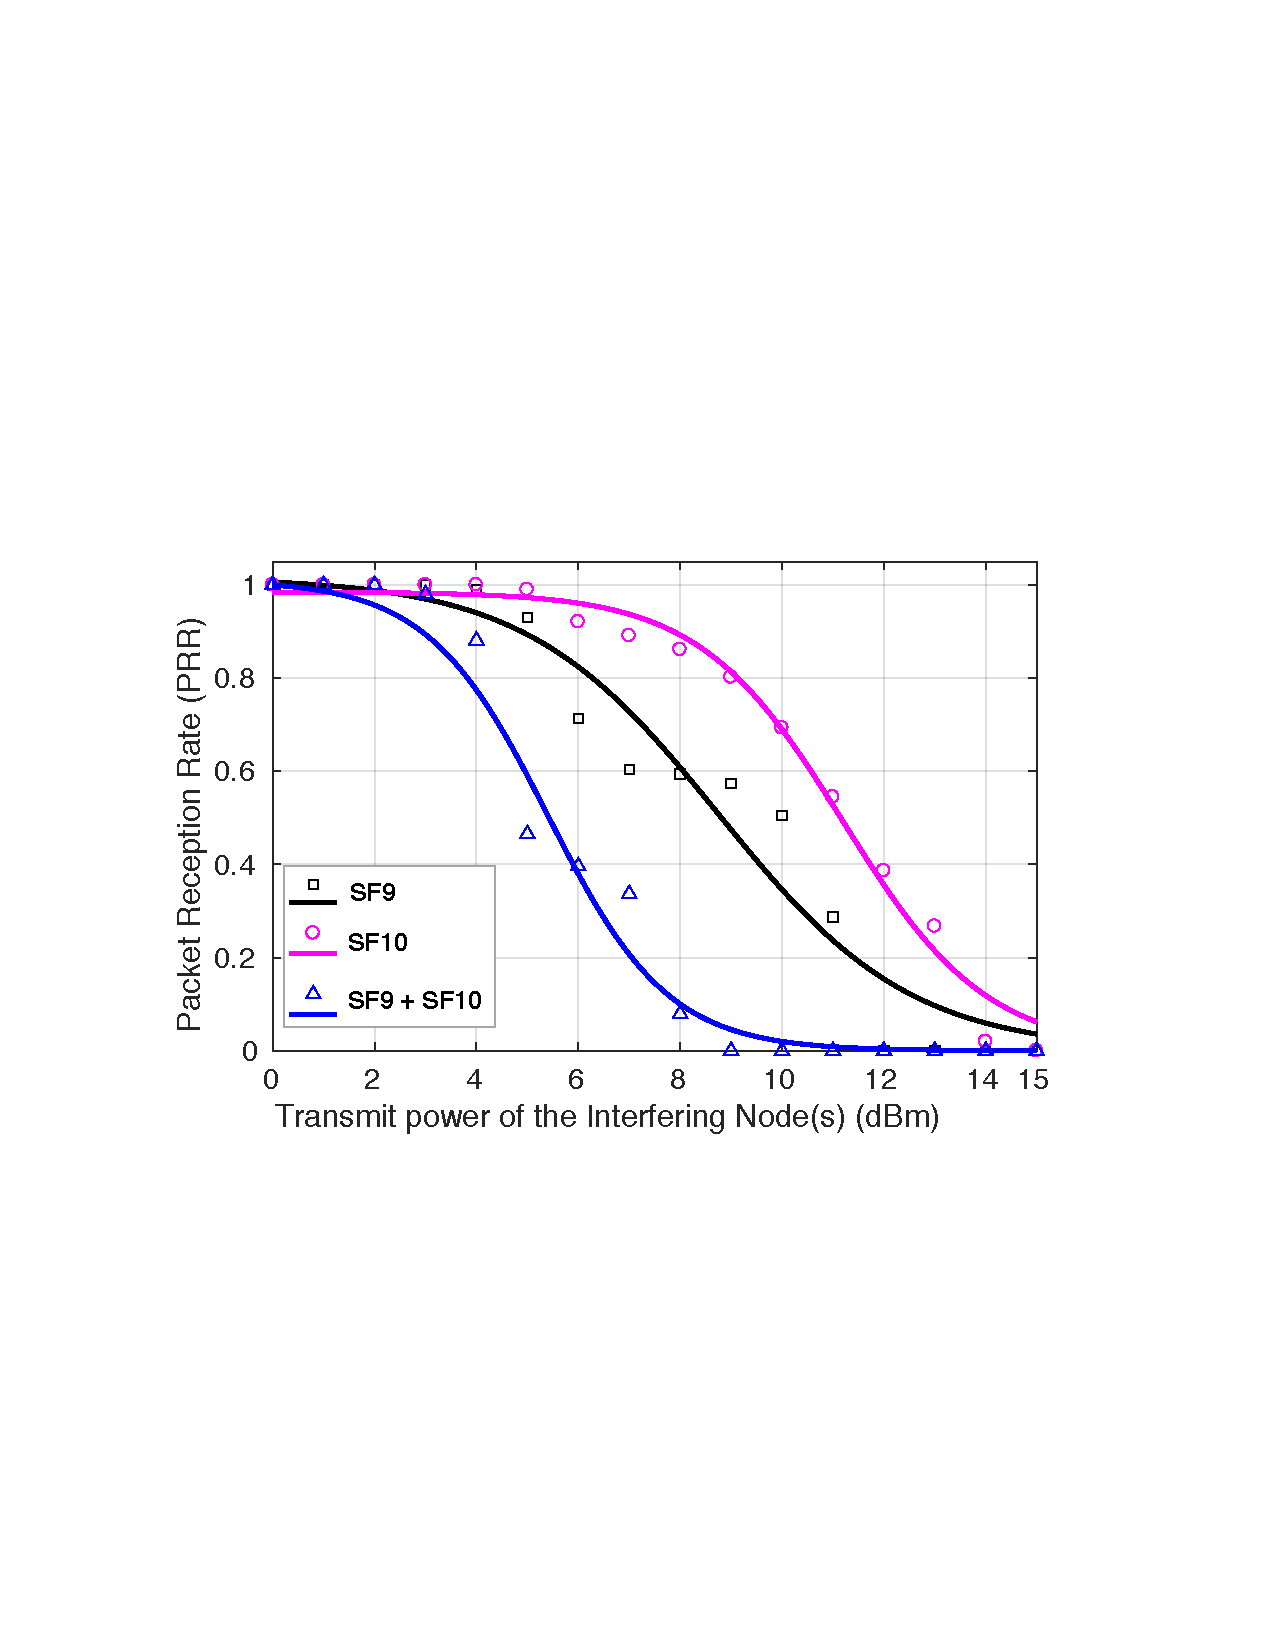
\includegraphics[width=0.8\columnwidth]{figures/aim-sf}
% \compactimg
% \caption{Packet Reception Rate (PRR) of packets sent at SF8 when overpowered by another transmission(s) on the same channel. We can also observe the additive interference caused by two simultaneous transmissions (SF9 and SF10).}
% \label{fig:aim-sf}
% \compactimg
% \end{figure}

% Our first experiment shows the interaction between different spreading factors as described by our additive interference model. Packets with varying configurations were sent out synchronously to force packet collisions and interference.
% LoRa devices are calibrated for receive power and placed at a distance of 3 $m$ from the gateway. 

% \figref{aim-sf} shows the packet reception rate of a node using spreading factor 8 (transmitting at 0 dBm) when sharing the same frequency with other node(s) using: spreading factor 9, 10 or both with increasing transmit power. Each data point was derived from 500 samples that fit the inverse sigmoid function. We can observe the additive interference and capture effect caused by the two transmitters which confirm the values presented by \cite{SemtechLoRaCommunity}.

%\begin{itemize}
%\item Capture effect 
%\item Spreading factor interaction (we can receive spreading factor with control)
%\end{itemize}

% \begin{figure*}[!bht]
% \centering

% \subfloat[]{
% \includegraphics[width=.24\linewidth]{figures/PairwiseDistance.pdf}
% } \hfill
% \subfloat[]{
% \includegraphics[width=.24\linewidth]{figures/PairwiseLocalization.pdf}
% } \hfill
% \subfloat[]{
% \includegraphics[width=.24\linewidth]{figures/InterfererDistance.pdf}
% } \hfill
% \subfloat[]{
% \includegraphics[width=.24\linewidth]{figures/InterfererLocalization.pdf}
% }
% \compactimg
% \caption{Depicts localization error results. (a) shows the error in measuring the distance between two points between our system and the RSSI baseline, which corresponds to the localization error shown in (b). (c) shows the error of our system in locating distances to a receiving-limited client, corresponding with the localization error shown in (d).}
% \label{fig:locres}
% \end{figure*}


% \subsection{Ranging and Localization} 
% In this experiment, we evaluate the performance of our localization and ranging experiments. We conduct our experiments on both indoor and outdoor spaces in a large university campus. Our testbed considers  30 randomly chosen client locations with pairs of clients separated by distances of up to 40 meters in settings composed of walls, furniture and other obtrusions between the radios. The maximum signal range afforded by the RTL SDR is 40~m, owing to its hardware not being optimized for the 400 and 900 MHz ISM bands. We consider two types of clients: (1) Powered clients that have access to channel state-information; (2) Transmit-only clients that do not provide channel state information, to emulate interferers or unsophisticated battery-powered LP-WAN radios.  We compare our system with a baseline that uses RSSI-based fingerprinting~\cite{rssi}. Note that unlike the baseline, our system does not assume prior fingerprinting of the environment. 

% \noindent\textbf{Locating Powered Devices}: We first measure the ranging error between pairs of clients that have access to channel-state information. Fig.~\ref{fig:locres}(a) depicts the CDF of the error in range between different pairs of devices whose distance is varied uniformly between 0-40 meters across randomly chosen locations in our indoor and outdoor testbeds. We observe a median ranging error of 2.21~m as against the RSSI baseline of 15.78~m. Fig.~\ref{fig:locres}(b) shows the CDF of the corresponding error in localization, recording a median error of 2.81~m as against the RSSI baseline of 16.81~m. We note that our approach achieves a superior accuracy in localization, despite the absence of prior fingerprinting of the environment, unlike the baseline. Further, while our maximum range with an RTL-SDR remains 40~m, owing to its general purpose design limited sensitivity to the 433~MHz/900MHz ISM bands, we believe our solutions error levels will remain consistent at full range with more sensitive RF front-ends optimized for these bands. 

% \noindent\textbf{Locating Interfering or Battery-Powered Radios}: Next, we  evaluate localization performance of radios that do not provide us channel state information (CSI). We measure the time-difference of arrival between such radios and two powered clients in our testbed that provide channel state information from three vantage points. We then measure the error in distance corresponding to this time-difference in arrival. We repeat our experiments with the distance between the radio and our clients ranging from 0-40 meters across randomly chosen locations in our indoor and outdoor testbeds. Fig.~\ref{fig:locres}(c) depicts the CDF of this error  with a median of 4.19~m. Fig.~\ref{fig:locres}(d) shows the CDF of the corresponding error in localization, depicting a median error of 4.20~m. These results demonstrate that our approach can locate both interfering devices and transmit-only radios with an accuracy of a few meters, despite not having access to transmitted data or channel state information from such devices.   


\subsection{Link Performance at the Whitespaces}
While the above experiments were performed on the open ISM frequencies (the 433 MHz band and 902-928 MHz), our approach can benefit from the opening up of additional frequencies in the TV whitespaces. Fortunately, commercial LoRa radios are capable of operating on the 512-572 MHz whitespace frequency bands. \figref{freq-rssi} plots the RSSI gathered by transmissions from one LP-WAN radio to another at a distance of three meters in a sealed anechoic chamber (for regulatory reasons). We observe that LoRa radio experiences a gradual drop in performance in the whitespace band, as frequencies withdraw from the 433~MHz band. This is quite natural given that the radios are designed for the ISM bands, and no low-cost radio can be expected to perform optimally across a wide range of sub-GHz frequencies. However, this shows the promise of deploying large-scale LP-WAN testbeds using current LoRa technology in the whitespaces, particularly in dense low-range scenarios, such as apartment complexes, where spectrum shortages are commonplace.  

\begin{figure}
\includegraphics[height=4.5cm]{figures/Freq_vs_RSSI.pdf}
\caption{Depicts the RSSI and signal-to-interference plus noise ratio (SINR) for two LoRa devices 3~m apart across frequencies, including the unlicensed and TV whitespace bands. Demonstrates commercial LoRaWAN radios can receive and transmit on the TV whitespaces.}
\label{fig:freq-rssi}
\compactimg
\end{figure}

% \begin{figure}[!htb]
% \centering
% \includegraphics[width=0.4\textwidth]{figures/snr_vs_freq.jpg}
% \includegraphics[width=0.4\textwidth]{figures/rssi_vs_freq.jpg}
% \compactimg
% \caption{{Depicts the RSSI and signal-to-interference plus noise ratio (SINR) for two LoRa devices three meters apart across frequencies, including the unlicensed 433 MHz, 902-918 MHz and the 512-572 MHz TV whitespace band. Demonstrates commercial LoRaWAN radios can receive and transmit on the TV whitespaces.   }}
% \label{fig:lorabug-power-trace}
% \compactimg
% \end{figure}


\subsection{Campus-wide deployment}

\begin{figure}[!hbt]
\centering
\includegraphics[width=\columnwidth]{figures/penetration_test_wean_cropped}
\compactimg
\caption{RF signal penetration experiments performed in a large poured-concrete building on campus. (left) shows the success rate for bi-directional packet exchange between end-node and gateway and (right) shows the RSSI at the gateway for successful transfers.}
\label{fig:penetration}
\compactimg
\end{figure}

% The remainder of this section describes the hardware and software components of our pilot network.

% \subsection{Server Back-end}

% The OpenChirp architecture shown in \figref{openchirp-arch} is a classical three-tiered design with sensor end-points at the bottom, followed by a gateway layer, and a server back-end that support applications at the top. All system configurations are carried out using a REST interface while devices that require more direct access to data like gateways or  processing agents communicate using a Publish-Subscribe layer.

% \noindent {\bf LoRaWAN Server:} The  LoRaWAN server is responsible for processing, decrypting and managing low-level LoRa communications. We extended the open-source LoRa server project~\cite{loraserver} that provides the underpinnings for MAC decisions like selection of the best downlink gateway, data rates and power levels for messages. The server exposes an MQTT-based Publish-Subscribe interface for both data and control messages making it easy to develop add-on modules. Most notably, we added support for our gateways hardware, our specific adaptive data rate algorithms and our global network management scheme.  

% \noindent {\bf Application Programming Interface (API):} External devices communicate with the OpenChirp network through two interfaces: (1) HTTP REST and (2) Publish-Subscribe (Pub-Sub). Client websites, mobile applications, management tools, etc. interface through an HTTP REST interface. The REST interface provides easy management of devices and their properties (location, metadata, functionality etc) as well as access to device time-series data. HTTP operations are managed by a server implemented in \textit{node}. Separating the OpenChirp API from the internal implementation of various services helps us create a modular architecture that also allows us to experiment with various components of the infrastructure.  

% \noindent {\bf Data Serialization:} A node can transfer limited data (tens of bytes per packet) over a LoRa connection due to a combination of communication restrictions and energy constraints. Data serialization gives us a flexible format to transfer various data types inside a single message structure. There are two observations with serialization: (1) the size for preregistered serialized messages is much smaller than if the same data were to be sent over raw key-value pairs and (2) existing serialization tools allow for faster processing and also enable static checking on serialized data. For the  serialization service, OpenChirp uses a simplified version of Google's Protocol Buffer~\cite{protobuff-google}, which can efficiently represent datatypes. When a new node is registered on the network, its serialization format is registered with the service. The service can then encode and decode data exchanged with the node.

% \noindent {\bf Timeseries and Meta-Data Storage:} A common application of IoT is identifying and acting on trends in the environment which requires data history. OpenChirp thus provides a time-series database (using \textit{InfluxDB}) that stores all data to and from end-devices. Applications and services can thus access historical data on-demand for a given time-interval in an efficient manner. This is accessible through our common REST API.  Some end-node and gateway properties like location, device type, capabilities, sensor sampling rates, closest gateway, etc. provide meaning and context to their data. These properties are stored as device metadata in an independent NoSQL (\textit{MongoDB}) database which also maintains access-control lists to regulate access to/modification of device data and meta-data. An LDAP authentication server is used to authenticate users that use the OpenChirp network. In our current deployment, students on campus can register and deploy their own devices with access control. If desired, they can share access with other account holders.


\begin{figure*}[!bt]
\centering
\subfloat{
\includegraphics[height=4cm]{figures/cmu_heatmap_wean.pdf}
} \hfill
\subfloat{
\includegraphics[height=4cm]{figures/cmu_heatmap_gsia.pdf}
} \hfill
\subfloat{
\includegraphics[height=4cm]{figures/cmu_heatmap_all_gw.pdf}
} \hfill
\subfloat{
\includegraphics[height=4cm]{figures/heatmap_scale.pdf}
}
\compactimg
\caption{Network coverage in and around a large university campus campus with rooftop base stations.  (left) and (middle) show coverage areas of two candidate gateways and (right) depicts that of the combination of all gateways.}
\label{fig:wardrive}
\compactimg
\end{figure*}


We currently have a campus-wide LoRaWAN system available to the student body deployed at a large university campus.  The system consists of four rooftop gateways that support a variety of custom and commercially available sensing devices.  Our base stations were deployed to support coverage of the complete geographical area as well as signal penetration inside buildings. After installing our four gateways, we perform a set of coverage tests. The tests are performed with a LoRa end-node configured for uplink communications with 125 kHz channel bandwidth, data rate of 980 bits/s, spreading factor of 10 and coding rate of $4/5$. Downlink communications from the gateway used 500 kHz channels at 3900 bits/s. \figref{wardrive} shows the coverage heatmap based on the average received signal strength indicator (RSSI) of $\sim 12$ messages sent from each location. Though some regions may not be covered using one gateway (due to shadowing, attenuation, etc.), a combination of four gateways can successfully cover all major campus regions (>6 square km). We also explored the penetration inside of buildings. \figref{penetration} shows the signal penetration across multiple floors of a large 250,000 sq.ft. 9-story poured concrete building with a single gateway located on the roof. The packet success rate on the left is computed based on the number of complete bi-directional transfers ($\sim 60$ points in each left corridor, $\sim 15$ points in each right corridor). The image on the right shows the gateway RSSI of successful transfers. The traces obtained from this testbed were used to drive the trace-driven simulations described below.

\begin{figure}[bth]
\centering
\includegraphics[width=0.8\columnwidth]{figures/8vs64channelvswhitespace}
\compactimg
\caption{Network throughput under increasing clients transmitting 20 byte packets every 15 minutes.  We see typical Aloha performance with a significant boost in capacity from a single White Space channel nearly matching the capacity of full 64-channel LoRaWAN gateway.}
\label{fig:ws-scaling}
\end{figure}

\section{Trace-Driven Simulations at Scale}
\label{sec:simulations}

Based on our micro-benchmarking experiments, we perform a set of trace-driven simulations to demonstrate the trends of our various approaches as the system scales.  \figref{ws-scaling} shows a baseline experiment simulating a week of time for a single base station in the middle of a 10$km$ by 10$km$ area with uniformly distributed nodes. The plot shows the effective throughput of the network as the number of clients increases using our additive interference model (spreading factor aware) as well as our more realistic capture effect model.  The 8-channel base-station represents the standard capacity of most current LoRa gateways.  The 64-channel base-station represents the capacity of our custom hardware which as one would expect servers approximately 8x more devices.  The 8-channel with a single white space band shows the potential of taking a normal gateway and equipping it with a white space radio system.  We see that each white space band provides about 80\% of the capacity of a 64-channel base station.  It is common for cities to have 1-3 of these bands free at any given time. 
 
% \subsection{Base-Station Management}
% \label{sec:bs-management}
% As the number of base-stations increase, the network must manage them so as to minimize interference due to uncoordinated devices. \figref{coloring} shows a simulated deployment with 50 base-stations and varying number of uniformly distributed devices. The devices transmit on a single frequency in any of the 8 available frequency sets, without frequency hopping and are set at a spreading factor of 10. Frequency set allocations used by base-stations for uplink are generated using a BFS graph coloring strategy. Two base-stations are considered neighbors in a graph if a transmission from any device can be received by both of them. If the number of colors in the colored graph exceeds 8 (the number of frequency sets), we break links corresponding to the longest distances until the graph is 8-colorable. This approach provides a 5\% improvement to data extraction rate over a random frequency assignment approach.

% \begin{figure}[bht]
% \centering
% \includegraphics[width=0.8\columnwidth]{figures/RandomVsColoring}
% \compactimg
% \caption{Performance of scheduled gateway frequencies as compared to a greedy-allocation. As load increases we see up to a 5\% improvement in overall capacity.}
% \label{fig:coloring}
% \compactimg
% \end{figure}


% \begin{figure}
% \includegraphics[width=0.8\columnwidth]{figures/binpacking}
% \caption{Performance of our load balancing approach using joint channel and spread-factor load balancing vs the currently adopted Greedy allocation. With uniformly distributed nodes, we see a 7\% improvement in capacity. }
% \label{fig:binpacking}
% \compactimg
% \end{figure}

% \subsection{Client to Base-Station Association}
% \figref{binpacking} shows the performance of our First-Fit bin packing heuristic, described in \secref{bs-assoc}, as compared with the commonly used greedy allocation scheme, that chooses to associate with the closest base-station. We simulate a dense deployment with 10 base-station (managed through coloring) in a small dense 1 $km^2$ area with other parameters identical to the previous section. As the density of nodes increases, the bin-packing scheme is better able to distribute the load between base-stations, reducing the number of collisions. The fact that we can utilize spreading factors to offload clients under heavy load is an interesting new technique for LP-WAN.

% \begin{figure}
% \includegraphics[height=4.5cm]{figures/InterferenceEstimation.jpg}
% \caption{Shows the increasing accuracy in detecting the number of clients impacted by interference, using measurements from an increasing number of wall-powered nodes.}
% \label{fig:intermit}
% \end{figure}

% \subsection{Interference Mitigation}\label{sec:resint}
% This section demonstrates our system's ability to crowd-source interference detection using a large number of wall powered nodes in the network. We simulate a wide-area deployment of 10,000 clients a subset of them, chosen uniformly at random, being powered-nodes. We then place an interferer at a randomly chosen location and estimate the number of nodes impacted by this interferer, using the bounds of the powered nodes as described in Sec.~\ref{sec:interferemit}.

% Fig.~\ref{fig:intermit} depicts the accuracy in the detection of impacted interferers as a function of the number of powered nodes. We observe that we can predict the impact of interference with $80\%$ accuracy with as few as $13\%$ of the clients in the network being wall-powered. 

% \begin{figure}
% \includegraphics[height=4.5cm]{figures/BaseStationCounter.jpg}
% \caption{Depicts the accuracy in detecting the number of clients a base station planned for a given location would serve, using measurements from an increasing number of wall-powered nodes in its vicinity. Using too many or too few nodes impacts accuracy. }
% \label{fig:netplan}
% \end{figure}

% \subsection{Network Planning}
% In this section, we evaluate the performance of the system in aiding base station deployment. We aim to calculate the number of nodes in range of a base station at a given location, prior to its deployment by using team of wall-powered clients to a emulate base station. We simulate a network of 10,000 nodes as before, with a 1\% of these nodes being powered. We assume the receive gain of powered nodes is $10\times$ weaker than that of the base station. We then calculate the accuracy of these nodes in tuning to the uplink and collectively measuring the number of clients in range of the base station.

% Fig.~\ref{fig:netplan} shows the percentage accuracy of this quantity against the number of wall-powered nodes employed to emulate the base station. We note that while using too few powered nodes is inaccurate, using too many causes estimates from nodes that are well beyond the range of the planned base station to be employed in is range estimate. The results reveal that the Goldilocks zone is about 10\% of all powered nodes, among those closest to the base station, which ensured an accuracy of 80\% in our estimate. 
